
%*****************************************
\chapter{Developing an Interaction System}\label{ch:forth}
%*****************************************

Introduce HCI and user-centered design\\

RECOGNITION RATHER THAN RECALL !!!\\


//add in why user centered design is so important for creating the interaction mechanism and in general?
// Consider the things needed to be considered in such a design: personas , ...
//Introduce the structure of this part: DESIGNING, TESTING, DEVELOPING \\

Make it clear that the interaction system was not meant for personal use, only for the purpose of the study.
Nevertheless we tried to adapt the development process as close to ucd and hci as possible in order to create a concept that is pleasant to use. 

\section {DESIGN}

\subsection{First Concept-Draft}

\begin{itemize}
\item create an interaction mechanism that presents a task which is modifiable in way to present the different ratios that we want to examine
\item The interaction could have presented any kind of interaction, yet creating a interaction system which resembled an authentication mechanism was more suitable.
\item that way the study participants are more able to put themselves in an authentication scenario when testing the system and answering the questions 
\item I had to think of a task that could be categorized into two sub-tasks. But first the user would have to memorize a certain sequence or combination. Then the first sub-task will be to think of the memorized combination - this represents the orientation phase. After that they would have to enter the combination - which is the active authentication time 
\item The task should be flexible in a way, such that different types of ratios are representable
\end{itemize}

\begin{enumerate}
    \item Short Orientation - Long active Authentication
    \item Long Orientation - Short Active Authentication
    \item Short Orientation - Short Active Authentication
\end{enumerate}

\begin{itemize}
\item the first design was inspired by the playfulness of Marbles and the Complexity of Pattern Rotation
\item the idea was that the user would be presented a certain pattern to memorize. This pattern consists of a certain number of nodes. Each node contains a certain image (emoji) inside of it. After memorizing, a 4x8 grid will be presented, which contains a collection of nodes, with images inside of them. 
\item each pattern begins with a node, which contains a key-symbol. 
\item in the orientation phase the user has to search for the correct key-node. When successfully found, they have to enter the pattern, by connecting the nodes in the correct order. 
\item in order to represent the different ratios of interest, each sub-task will be modified in a certain way:
    
\begin{itemize}
\item Short Orientation: In order to present short orientation the grid will only contain one node that contains a key symbol. That way, searching and finding the correct pattern will be obvious and easy for the user and will not take a long time 
\item Long Orientation: The Grid will contain multiple nodes that contain a key, making the search task more challenging for the user, so it takes longer to find the correct one. 
\item Short Active Authentication: user has to memorize an easy and short pattern
\item Long Active Authentication: user has to memorize a complicated and long pattern 
\end{itemize}

POINT OUT WHAT YOU DID NOT LIKE ABOUT THE DESIGN AND WHAT YOU THEREFORE CHANGED ! 

\begin{figure}[H]
\begin{center}
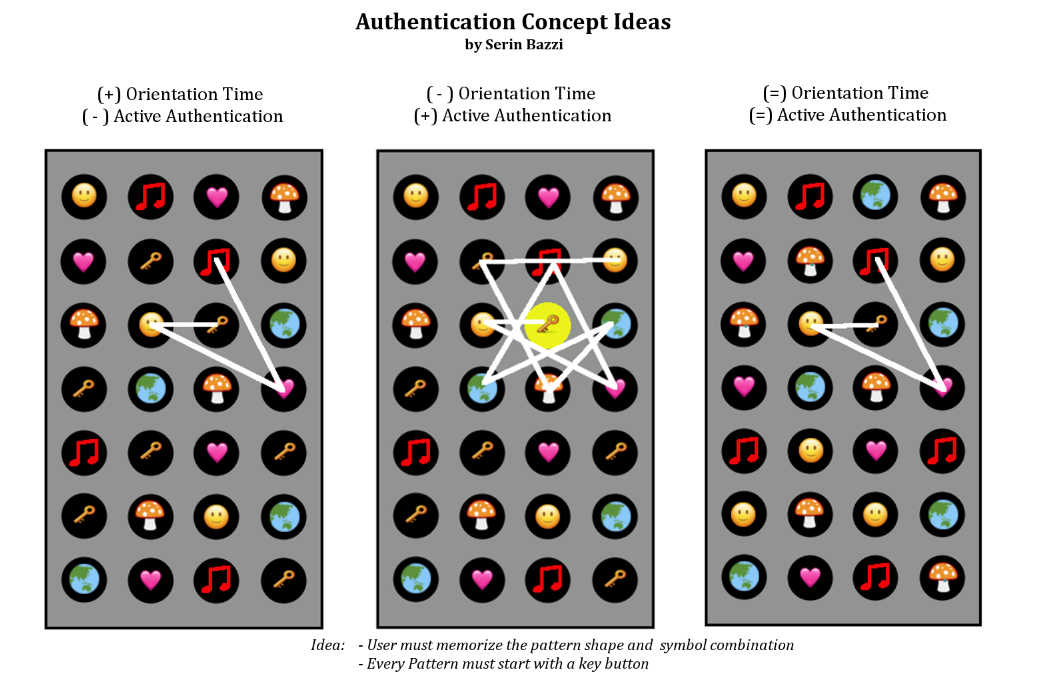
\includegraphics[width=130mm,height=70mm]{Chapters/graphics/Sketch.PNG}
\caption{}
\label{drawing}
\end{center}
\end{figure}

\subsection{Second Concept-Design}
\item after testing the concept out on a paper prototype , realized that the many symbols were perceived overwhelming and confusing 
\item Therefore, we decided to use simple shapes instead of images/emojis, BECAUSE SHAPES ARE MUCH MORE MEMORABLE FOR HUMAN BEINGS 
\item Furthermore, we changed the color of the node itself. It could be either Green, Blue or Red. For a simplistic design we stayed with the NATURAL COLORS OF THE HUMANS EYE
\item Then I also made the grid a bit smaller (from 4x7 to a 4x8)
\item Each pattern would begin with a red node containing a triangle shape. RED BECAUSE ALERTING , TRIANGLE ?? 
\item this time the pattern is less complex, which makes it easier for the user to memorize and remember. Instead of the having X different images the nodes may only contain 1 of three different shapes. The first node is the only node in the pattern that is red and that contains a triangle. The rest are either green or blue and contain either a square or a circle shape. 
\item another modification made is the way in which the pattern is entered. In design one we wanted the pattern to be entered in a swiping manner. Although it may be more suitable interaction, since the user is working on a touch display, it is a fast option of input. For the sake of the study, we opted for a input-technique by pressing the nodes, in order to be able to create a long active authentication phase, without having to complicate the pattern to do so. 

\item Short Orientation: a grid will contain multiple blue and green nodes and only one red node containing a triangle. That way the position of the pattern is obvious and the user can find it in a short time 
\item Long Orientation : a grid will contain multiple (how many?) red nodes with triangles and the user has to find the correct red node to enter the pattern
\item Short Input: a short pattern consisting of 4 nodes and requires only 4 presses 
\item Long Input: a long pattern consisting of 5 nodes and requiring 10 presses 
\item ADD PICTURE HERE OF DESIGN
\item EXACTLY EXPLAIN THE STRUCTURE OF THE TASK

\section{TESTING}

\item The design was tested using a paper prototype of the concept.
\item Important points to consider were the overall asthetic of the design
\item the memorability of the patterns 
\item and the time each of the phases takes 
\item there were 6 participants in the testing 
\item whilst testing the concept, the time was measured using a stop watch 
\item in order to estimate the time needed for Long/Short Orientation and Input, the time intervall between the moment when the user was shown the grid and the time when they placed their finger on the first node of the pattern, signalised the orientation
\item then the time between the selection of the first node and the selection of the last node, signalised the input. 
\end{itemize}
INSERT TIME MEASUREMENTS HERE !!! 

\section {DEVELOPING}
\begin{itemize}
\item Before developing the Concept as an App, the concept was first pitched to the Professor by presenting a walkthrough of the App using a Paperprototype
\item the walkthrough was also developed in order to create a structure I could base myself on, whilst developing the App. Although the structure got modified along the way, having a grobe Vorstellung hilft waehrend der Entwicklung.
\item PRESENT A WALKTHROUGH OF THE APP HERE 
\item Creating the Grids: I decided to design the grid by hand for many reasons 
\item 1, so that I make sure that my pattern is contained in the Grid only once, which my not be the case with randomization
\item 2. so that I could complicate the Long Orientation Phase, by placing in many nodes similar to the ones in the pattern, in order to create confusion
\item The Concept was developed into an app using Android Studio. 
\item Time Measurement: 
\item in order to measure the time I had to think of a way to measure the exact time it takes the user to find the pattern and the exact time it takes to enter the pattern 
\item in the paper they orientation time was measured as soon as the phone screen turned on
\item the environment in the study will be more different, since the user will always have the feeling and by feeling put under pressure they will preform differently than in the real world
\item Although it would make sense to start the measurement of the orientation time as soon as the grid is presented, it would become overwhelming for the user, considering they would have to fulfill the task 3 times in a row. 
\item therefore I decided to add a start button before each grid, such that the user can mentally prepare himself for the upcoming task. 
\item adding the start button also guaranteed getting exact orientation times, because the user knew that as soon as the button was pressed, they had to concentrate. No pause created by overwhelm or surprise that another task follows, affected the orientation time during the study
\item The measurement of the orientation began after the Start Button was pressed and ended as soon as the correct red node in the grid was pressed 
\item In the paper measuring the input time started with the first input and ended with the last 
\item considering that in this case the task is not only one easy authentication and that the participant is required to fulfill a number of small tasks one after the other, there is a possibility of loosing focus of concentration 
BACK THIS UP WITH SOME SCIENTIFIC FACTS ??
Therefore I decided to not connect the measurements as in the paper and strictly divide these two times from each other. 
\item after the participant would find the correct pattern, another grid is displayed in which all of the nodes, expect for the ones, needed for the input are blended out. 
That way they can solely focus on the pattern without being distracted by the other nodes in the grid. 
\item for the input the first node in the pattern must be included, although it was pressed before, but that only counted to signalize that the pattern was found. 
\item this structure ensured a clean and exact measurement of the two phases. 

\item Structure of the APP: in phases and levels and patterns , considering 3 levels , whereby the 3rd is the actual one we will observe. 

\item testing out the app, adding a training segment, including a reminder pop (error recovery), the failed input trial is not considered 

\end{itemize}

